% This is a LaTeX thesis template for Monash University.
% to be used with Rmarkdown
% This template was produced by Rob Hyndman
% Version: 6 September 2016

\documentclass{monashthesis}

%%%%%%%%%%%%%%%%%%%%%%%%%%%%%%%%%%%%%%%%%%%%%%%%%%%%%%%%%%%%%%%
% Add any LaTeX packages and other preamble here if required
%%%%%%%%%%%%%%%%%%%%%%%%%%%%%%%%%%%%%%%%%%%%%%%%%%%%%%%%%%%%%%%

\author{Xiefei Li}
\title{Revisiting the Forecast Combination Puzzle: An Empirical Study}
\studentid{30204232}
\studentemail{\href{mailto:xlii0145@student.monash.edu}{\nolinkurl{xlii0145@student.monash.edu}}}
\studentdetails{Supervisor: David T. Frazier}
\supervisoremail{\href{mailto:David.frazier@monash.edu}{\nolinkurl{David.frazier@monash.edu}}}
\def\degreetitle{Bachelor of Commerce (Honours)}
% Add subject and keywords below
\hypersetup{
     %pdfsubject={The Subject},
     %pdfkeywords={Some Keywords},
     pdfauthor={Xiefei Li},
     pdftitle={Revisiting the Forecast Combination Puzzle: An Empirical Study},
     pdfproducer={Bookdown with LaTeX}
}


\bibliography{thesisrefs}

\begin{document}

\pagenumbering{roman}

\titlepage

{\setstretch{1.2}\sf\tighttoc\doublespacing}

\clearpage\pagenumbering{arabic}\setcounter{page}{1}

\hypertarget{abstract}{%
\chapter*{Abstract}\label{abstract}}
\addcontentsline{toc}{chapter}{Abstract}

The abstract should outline the main approach and findings of the thesis and must not be more than 500 words.

Finish up afterwards.

\newpage

\hypertarget{acknowledgements}{%
\chapter*{Acknowledgements}\label{acknowledgements}}
\addcontentsline{toc}{chapter}{Acknowledgements}

I would like to thank my supervisor, my Honours coordinator, all the people who helped me throughout the year and myself.

\hypertarget{introduction}{%
\chapter{Introduction}\label{introduction}}

\hypertarget{research-objective}{%
\section{Research Objective}\label{research-objective}}

This thesis aims to investigate the determinants behind, and evidence for the forecast combination puzzle in various domains, and to empirically examine a general solution to the forecast combination puzzle. The combination puzzle refers to the well-known empirical finding that an equally weighted combination of forecasts generally outperforms more sophisticated combination schemes. This phenomenon is often found in the point forecast combinations but it is also the case in the density forecast combinations. Starting with two different types of time series datasets, this paper explores how the in-sample performance of the constituent models influences the presence of the puzzle. The empirical studies undertaken so far have focused more on pure time series settings, while there is little literature on the puzzle in the cross-sectional setting. A simulated study is designed to investigate the puzzle in the two-model combination under a regression analysis. The performance of density combinations will be assessed via the log score function and the mean squared forecast error will be used to assess the point combinations for seasonal data. As an additional contribution, we will assess the veracity, and applicability, of a recently proposed solution to the forecast combination puzzle suggested in \textcite{ZMFP22} and \textcite{FZMP23}.

\hypertarget{literature-review-and-motivation}{%
\section{Literature Review and Motivation}\label{literature-review-and-motivation}}

The forecast accuracy is of critical concern for forecasters and decision makers. With the evidence of dramatic improvements in the forecast accuracy, forecast combinations have attracted wide attention and contributions in the literature, both theoretical and applied \autocite{C89,T06}. More importantly, this promising approach often has a robust performance for various types of series, proved by numerous empirical results \autocite{GA11}. \textcite{MACF82} carefully examined the forecast accuracy with a considerable amount of time series, and reported that forecast combinations perform better than individual models. Later, \textcite{SW98} claimed that the best-performing single forecast can be further improved by incorporating other forecasts, based on their empirical comparisons of different forecasting methods. Despite of point forecasting, researchers also devote efforts on probabilistic forecasting to obtain more information about uncertainties. They also keep finding that density forecast combination outperforms individual density forecast \autocites[e.g.,][]{HM07,GA11}.

Forecast combinations refer to the idea of combining multiple forecasts generated from possible models, which was originally proposed in the seminal work of \textcite{BG69}. The forecast combination methods, in general, involve producing forecasts from constituent models, and then combining them based on a rule or weighting scheme. Each scheme has different selection criteria for the ``best'' forecast combination and the corresponding weight value assigned to each model. This process can sometimes capture more meaningful characteristics of the true data generating process than using a single model, and allow us to combine the best features of different models within a single framework. Researchers have examined a variety of combination methods for both point and density forecasts over the past 50 years, see \textcite{WHLK22} for a modern literature review.

In most time series setting under which forecast combinations are employed, a striking empirical phenomenon is often observed, coined by \textcite{SW04}, as the ``forecast combination puzzle''. The puzzle is encapsulated by the fact that ``theoretically sophisticated weighting schemes should provide more benefits than the simple average from forecast combination, while empirically the simple average has been continuously found to dominate more complicated approaches to combining forecasts'' \autocite{WHLK22}. In other words, complex weighting schemes are designed to improve the accuracy, so these refined forecast combinations should perform better in theory. However, the mean of the contemporaneous forecasts appears to be more robust in practice than weighted forecasts combined through complicated schemes. This finding has been continuously reaffirmed by extensive literature reviews and papers \autocites[e.g.,][]{C89,SW98,SW04,SW09,MSA18,MSA20}, and the simple averaging naturally becomes a benchmark.

There are two possible explanations for the puzzle in the literature. One concentrates on the estimation uncertainty in combination weight \autocite{SW98,SW04,SW09}. Complicated weighting schemes introduce variability and uncertainty when estimating parameters, whereas the simple averaging does not require any estimation. The higher average loss and instability in the study of \textcite{SW04} were a strong evidence for the inferior performance of sophisticated weighting schemes. On the other hand, \textcite{E11} and \textcite{CMVW16} explore the trade-off between bias and variance in the Mean Squared Forecast Error (MSFE). \textcite{CMVW16} demonstrated the presence of bias and inefficiency when weights estimation is required, in comparison with the fixed-weights such as the equal weights. They further proved that equally weighted combination is unbiased and its variance has only one component, resulting in a smaller mean squared error than a biased combination. However, this is applicable and specific to the MSFE scheme. Furthermore, the underlying implication or condition of these explanations is that the puzzle must be found in each particular circumstance, which has not been rigorously demonstrated in theory. As a result, we will take a step back and focus on systematically exploring when the puzzle will be evidenced. In other words, when should we expect the puzzle to appear?

Consider a simple case of two-model combination, the initial conjecture is that the presence of the puzzle is highly related to the in-sample fit of two constituent models. When both models fit the data well or bad, the puzzle is likely to happen. If only one of them fails to capture the data patterns, the optimal forecast combination will give more weight on the better one, but the puzzle is ambiguous. The simple average forecast can perform much better than the optimal combination forecast, or vice versa. Table \ref{tab:1} visually summarizes this hypothesis.

\begin{table}[ht]
\centering
\begin{tabular}{cccc}
                       &      & \multicolumn{2}{c}{$M_2$} \\
                       &      & Good       & Bad       \\
\multirow{2}{*}{$M_1$} & Good & $\surd$    & $?$ \\
                       & Bad  & $?$        & $\surd$
\end{tabular}
\caption{The first row and the first column refer to two constituent models in a combination, $M_1$ and $M_2$. ``Good`` means that the model fits the data well, whereas ``Bad`` denotes that the model fails capture some important features of the data. The ``$\surd$`` implies the presense of the forecast combination puzzle, while ``$?$`` means the forecast combination puzzle is uncertain.}
\label{tab:1}
\end{table}

More specifically, when the accuracy of in-sample fit for two models are very similar, then two models are both \texttt{Good} or both \texttt{Bad}, which are the diagonal cases in Table \ref{tab:1}. It is possible that two models perform equally bad but for different reasons. In terms of the off-diagonal cases, a \texttt{Good} model fit and a \texttt{Bad} model fit are determined in a relative sense, i.e., one model fits the data far more superior than the other. This can be indicated by the apparent difference in the in-sample accuracy between two models.

Even though there is a widespread literature among different pure time series settings, no attention appears to have been given to the cross-sectional setting. We investigate the forecasting performance of two-model pools for the cross-sectional data in the linear regression form via a simulation study. We have found that the evidence of the forecast combination puzzle is not just about the fit of constituent models but the interaction of the model with the DGP. Mainly focused elements are the sample size, the true value of parameters except the intercept, and the variances of regressors. The advantages of using simulation are that the true DGP is known and we can easily manipulate values to see any interesting changes. This study also provides sufficient empirical evidence to better examine or support our conjecture in Table \ref{tab:1}. In addition, the regression form is easy to understand and analyse how various parts interact with each other. For example, it is known that the in-sample fit of a linear regression model can be represented by \(R^2\), which is therefore a suitable measure to determine \texttt{Good} and \texttt{Bad} models in this context.

While various explanations for the forecast combination puzzle have been suggested over the years (see the above references), a general solution to the puzzle has so far proved elusive. Recently, \textcite{ZMFP22} and \textcite{FZMP23} proposed a new explanation for the puzzle in a general way by investigating the sampling variability of the forecasts induced via estimation of the constituent model forecasts (i.e., the models used to produce the forecasts). They illustrated that, asymptotically, the bias and variability mainly come from the estimation of the models used to produce the constituent model forecasts. The common way of producing forecast combinations keeps the model estimation uncertainty fixed during the weight estimation process, which is one reason of having the puzzle. If constituent models and weights can be estimated jointly, if feasible, the puzzle can be eliminated suggested by \textcite{FZMP23}. Under this approach, the sophisticated weighting schemes should (asymptotically) be superior.

The goal of this thesis is manifolds: first, to substantiate the presence of the combination puzzle in the usual time series in which it has been found; second, to explore the relationship between the puzzle and the in-sample fit of constituent models; third, to search for empirical evidence of the combination puzzle in cross-sectional settings; fourth, to test the empirical veracity of the theoretical solution to the puzzle found in \textcite{FZMP23}, both within, and outside of, the standard time series setting where the puzzle is often observed.

\hypertarget{method}{%
\chapter{Methodology}\label{method}}

The first goal of this paper is to construct linear density forecast combinations with parametric models. The results are anticipated to reveal that forecast combinations can deliver improved accuracy over single models, but are not necessarily superior to forecasts obtained from the equally weighted combination.

Next, we will investigate the effect of in-sample performance between two constituent models on the presence of the forecast combination puzzle empirically. One way of badly fit the dataset is to simply ignore the important features of the data in the model specification. Two main scenarios are considered: a small difference of the in-sample accuracy and a big difference of the in-sample accuracy.

The last goal is to estimate the unknown parameters of the constituent models and the weight in a single step, and to compare the accuracy of forecasts based on these combinations against the usual combinations process, as well as the equally weighted combination. To measure differences between these forecasts, we will eventually employ forecast accuracy tests, of the type derived in \textcite{W96}, which measure out-of-sample differences between forecasts.

In the literature, there are several definitions of combinations. We focus on the combination of forecasts from independent models for a given dataset, which is commonly performed in two stages:

\begin{enumerate}
\def\labelenumi{\arabic{enumi}.}
\item
  producing separate point or probabilistic forecasts for the next time point using observed data and constituent models, and
\item
  combining forecasts based on one of the accuracy criteria.
\end{enumerate}

Specifically, we only consider the combination of two individual forecasts, which allows us to delve into interesting and unexplained findings through fast data manipulation.

Before explaining further details, the following notation will be used throughout the paper. A vector time series \(\textbf{y}_t\) with a total of \(T\) observations will be divided proportionally into two parts, an in-sample period \(R\) and an out-of-sample period \(P\). The realization of a target variable \(y\) at time \(t\) is denoted as \(y_{t}\). Its future values after the in-sample period is denoted as \(y_{\small{R+h}}\), where \(h\) is the forecast horizon and \(h>0\). The information set at time t, \(\mathcal{F}_t\), is comprised of all observed (and known) realizations of \(y\) up to time t, i.e., \(\mathcal{F}_t = \{y_1, y_2, .., y_t\}\).

The specifications of constituent models are determined by the features of the in-sample data. For each model, the error term is assumed to be independent and normally distributed so that the Maximum Likelihood Estimation (MLE) method can be applied to generate the estimators of unknown parameters. Given the log likelihood function of in-sample period for each model, the corresponding estimates are obtained when they maximize that function and then held fixed for the following procedures. The optimal combination is then constructed with the estimated weight of each model that delivers the best accuracy.

A parametric model \(M\) determines the conditional probability density for \(\textbf{y}_t\), denoted by \(f(y_t|\mathcal{F}_{t-1}, \theta_M, M)\), given unknown parameters \(\theta_M\) and all the past information \(\mathcal{F}_{t-1}\). The choice and specification of constituent models vary by the features of the in-sample data. For each model, the error term is assumed to be independent and normally distributed so that the Maximum Likelihood Estimation (MLE) method can be applied to generate the estimators of unknown parameters, i.e., \(\hat\theta_M = \underset{\theta_M}{\arg\max} \sum^R_{t=1} log f(y_t|\mathcal{F}_{t-1}, M)\). Given the log likelihood function of in-sample period for each model, the corresponding estimates are obtained when they maximize that function and then held fixed for the following procedures.

\hypertarget{density-combinations}{%
\section{Density combinations}\label{density-combinations}}

\hypertarget{linear-pooling}{%
\subsection{Linear pooling}\label{linear-pooling}}

Consider the case of only two competing probability densities, undoubtedly, densities can be combined in many ways; see Section 3 of \textcite{WHLK22} for many popular means of probabilistic combination. One of the commonly used approaches is the ``linear opinion pool'': aggregate constituent weighted densities in a linear form \autocites[e.g.,][]{BG69,HM07,GA11}. For the \texttt{two-model} pools, constituent densities \(f_1(y_t)\) and \(f_2(y_t)\) are combined as follows:

\begin{equation}
\label{eqn:LC1}
f(y_t) = w \ f_1(y_t | \mathcal{F}_{t-1}, \hat\theta_{M1}, M_1) + (1-w) f_2(y_t | \mathcal{F}_{t-1}, \hat\theta_{M2}, M_2)
\end{equation}

where \(w\) is the non-negative weight allocated to the probability density derived from the first model. Through this construction, the sum of two weights is implied to be 1, which is a necessary and sufficient condition for \(f(y_t)\) to be a proper density function \autocite{GA11}. In addition to point forecasts, the use of density forecasts can offer forecasters or decision markers a more comprehensive view of the target variable (see section 2.6.1. of \textcite{FTP22} for related contributions).

\hypertarget{log-socring-rules}{%
\subsection{Log socring rules}\label{log-socring-rules}}

Following the literature on density evaluation, our initial analysis will focus on using the log score function to measure the accuracy of our density forecasts; see, e.g., \textcite{GA11} for a discussion on log score and its use in density forecasting. For each individual model \(M\), the log score over the sample \(t = 1, \dots, T\) is:

\begin{equation}
\label{eqn:LS1}
LS = \sum^T_{t=1} log \ f(y_t| \mathcal{F}_{t-1}, \hat\theta_M, M).
\end{equation}

The ``optimal'' linear combination is identified to produce the most accurate forecasts when the set of weights maximizes the log score function of two densities over the in-sample \(t = 1, 2, \dots, R\).

\begin{equation}
\label{eqn:LS2}
\hat{w}_{\text{opt}} = \underset{w}{\arg\max} \sum^R_{t=1} log \Big[ w \ f_1(y_t| \mathcal{F}_{t-1}, \hat\theta_{M1}, M_1) + (1-w) \ f_2(y_t| \mathcal{F}_{t-1}, \hat\theta_{M2}, M_2)\Big]
\end{equation}

Thus, the log predictive score over the forecast horizon \(h = 1, 2, \dots, P\) (i.e., the out-of-sample period) is:

\begin{equation}
\label{eqn:LS3}
LPS = \sum^T_{t = R+1} log \Big[ \hat{w}_{\text{opt}} \ f_1(y_t| \mathcal{F}_{t-1}, \hat\theta_{M1}, M_1) + (1- \hat{w}_{\text{opt}}) \ f_2(y_t| \mathcal{F}_{t-1}, \hat\theta_{M2}, M_2)\Big].
\end{equation}

\hypertarget{point-combinations}{%
\section{Point combinations}\label{point-combinations}}

Although our main focus is the density forecast combination, to save time and make the evaluation easier, the point forecast combination is also used but only for the seasonal time series. The point forecast of each model corresponds to the mean value of the predicted density distribution. We will use the mean squared forecast error (MSFE), following \textcite{BG69} and \textcite{SW09}, to measure the accuracy of point forecast combinations in the two-model pools.

\hypertarget{linear-combination}{%
\subsection{Linear combination}\label{linear-combination}}

Similar to the density case, point predictions from two constituent models, \(\hat y_{1t}\) and \(\hat y_{2t}\), are aggregated linearly:

\begin{equation}
\label{eqn:PC1}
\hat y_t = w \ \hat y_{1t} + (1-w) \ \hat y_{2t}
\end{equation}

where \(w\) is the non-negative weight allocated to the point prediction generated from the first model.

\hypertarget{mean-squared-forecast-error}{%
\subsection{Mean squared forecast error}\label{mean-squared-forecast-error}}

The MSFE of an individual model is the average of squared difference between the actual value and the predicted value at each time point over the in-sample period \(R\):

\begin{equation}
\label{eqn:MSFE1}
\frac{1}{R} \sum^R_{t=1} (y_t - \hat y_t)^2.
\end{equation}

The lower the MSFE, the better the performance. Therefore, the ``optimal'' set of weights satisfies that it minimizes the MSFE of the point forecast combination among all other possible sets over the training period.

\begin{equation}
\label{eqn:MSFE2}
\hat{w}_{\text{opt}} = \underset{w}{\arg\min} \frac{1}{R} \sum^R_{t=1} w \ \hat y_{1t} + (1-w) \ \hat y_{2t}
\end{equation}

Consequently, the MSFE over the evaluation horizon \(h = 1, 2, \dots, P\) is:

\begin{equation}
\label{eqn:MSFE3}
MSFE = \frac{1}{P} \sum^T_{t = R+1} \hat{w}_{\text{opt}} \ \hat y_{1t} + (1-\hat{w}_{\text{opt}}) \ \hat y_{2t}.
\end{equation}

\hypertarget{empirical-results}{%
\chapter{Empirical Results}\label{empirical-results}}

\hypertarget{sp500}{%
\section{Pure time series setting (S\&P 500)}\label{sp500}}

Reconsidering the example in Section 3 of \textcite{GA11}, the data we use is the daily Standard and Poor's (S\&P) 500 index from February 11, 2013 to February 10, 2023 (10 years in total), retrieved from the \textcite{SP500}. The S\&P 500 index dataset has a total of 2519 (\(T\)) observations and is partitioned into two periods with a rough proportion. The in-sample period contains the first 60\% of the data (\(R = 1511\)), which is used to estimate all unknown parameters, including the optimal weight. The remaining 40\% (\(P = 1008\)) becomes the out-of-sample period to evaluate the forecast performance.

We will investigate the presence of the forecast combination puzzle when both models fit the training set well and when one of the model badly fit the data. Constituent models are based on common classes of models: autoregressive integrated moving average (ARIMA), exponential smoothing (ETS), and linear regression model with ARIMA errors. Detailed model specifications for each case will be elaborated in the Appendix.

We choose three prediction models to study the performance of density predictions across sets of \texttt{two-model} pools. Each of the \(j\) predictive model has a conditional Gaussian density, which takes the form \(f^{(j)}(y)=f_j(y_t|\mathcal{F}_{t-1})=N\{y_t; \mu_j, \sigma^2_j\}\), where \(N\{x; \mu, \sigma^2\}\) denotes the normal probability density function evaluated at value \(x\) with mean \(\mu\) and variance \(\sigma^2\). The notation \(\mathcal{F}_{t-1}\) denotes all information available at time \(t-1\), and we assume that the conditional mean and variance of the models are, up to unknown parameters, known at time \(t-1\).

\hypertarget{nonstationary-time-series}{%
\subsection{Nonstationary time series}\label{nonstationary-time-series}}

To reduce the level of variability, we take a natural logarithm of the S\&P 500 index \(y_t\) and fit the data directly without removing its stochastic trend with three candidate models. There are three sets of two-model combinations in total. Consider the weight \(w\) takes a value from 0 to 1 and changes by 0.01 every time. The log score, as a function of weight, is generated to search for the optimal weight over the in-sample \(R\) period (refer to the top row of Figure \ref{fig:nonstat}). According to equation \ref{eqn:LS2}, the estimated optimal weight corresponds to the maximum point of the curve. Then we can calculate the log predictive score of the optimal combination for the out-of-sample period based on equation \ref{eqn:LS3}.

\begin{table}[ht]
  \centering
    \begin{tabular}{l|ccc}
    \toprule
                                      &    Left     &   Middle    &    Right   \\
    \midrule
    In-sample log score difference    &   5.8989    &   1.2718    &   7.1707   \\
    Optimal versus average            &   9.9569    &   0.2268    &  19.9928   \\
    Presence of the puzzle            &   Yes       &   Yes       &   Yes      \\
    \bottomrule
    \end{tabular}
  \caption{``Left``, ``Middle`` and ``Right`` correspond to the position of each pair of combination in Figure \ref{fig:nonstat}. ``In-sample log score difference`` denotes the absolute difference of the log score over the training period between two models, which can be viewed as an informal accuracy measure of in-sample fit. ``Optimal versus average`` shows the absolute difference in log predictive score between the optimal combination and the simple average.}
  \label{tab:comparison1}
\end{table}

\begin{figure}[ht]
\centering
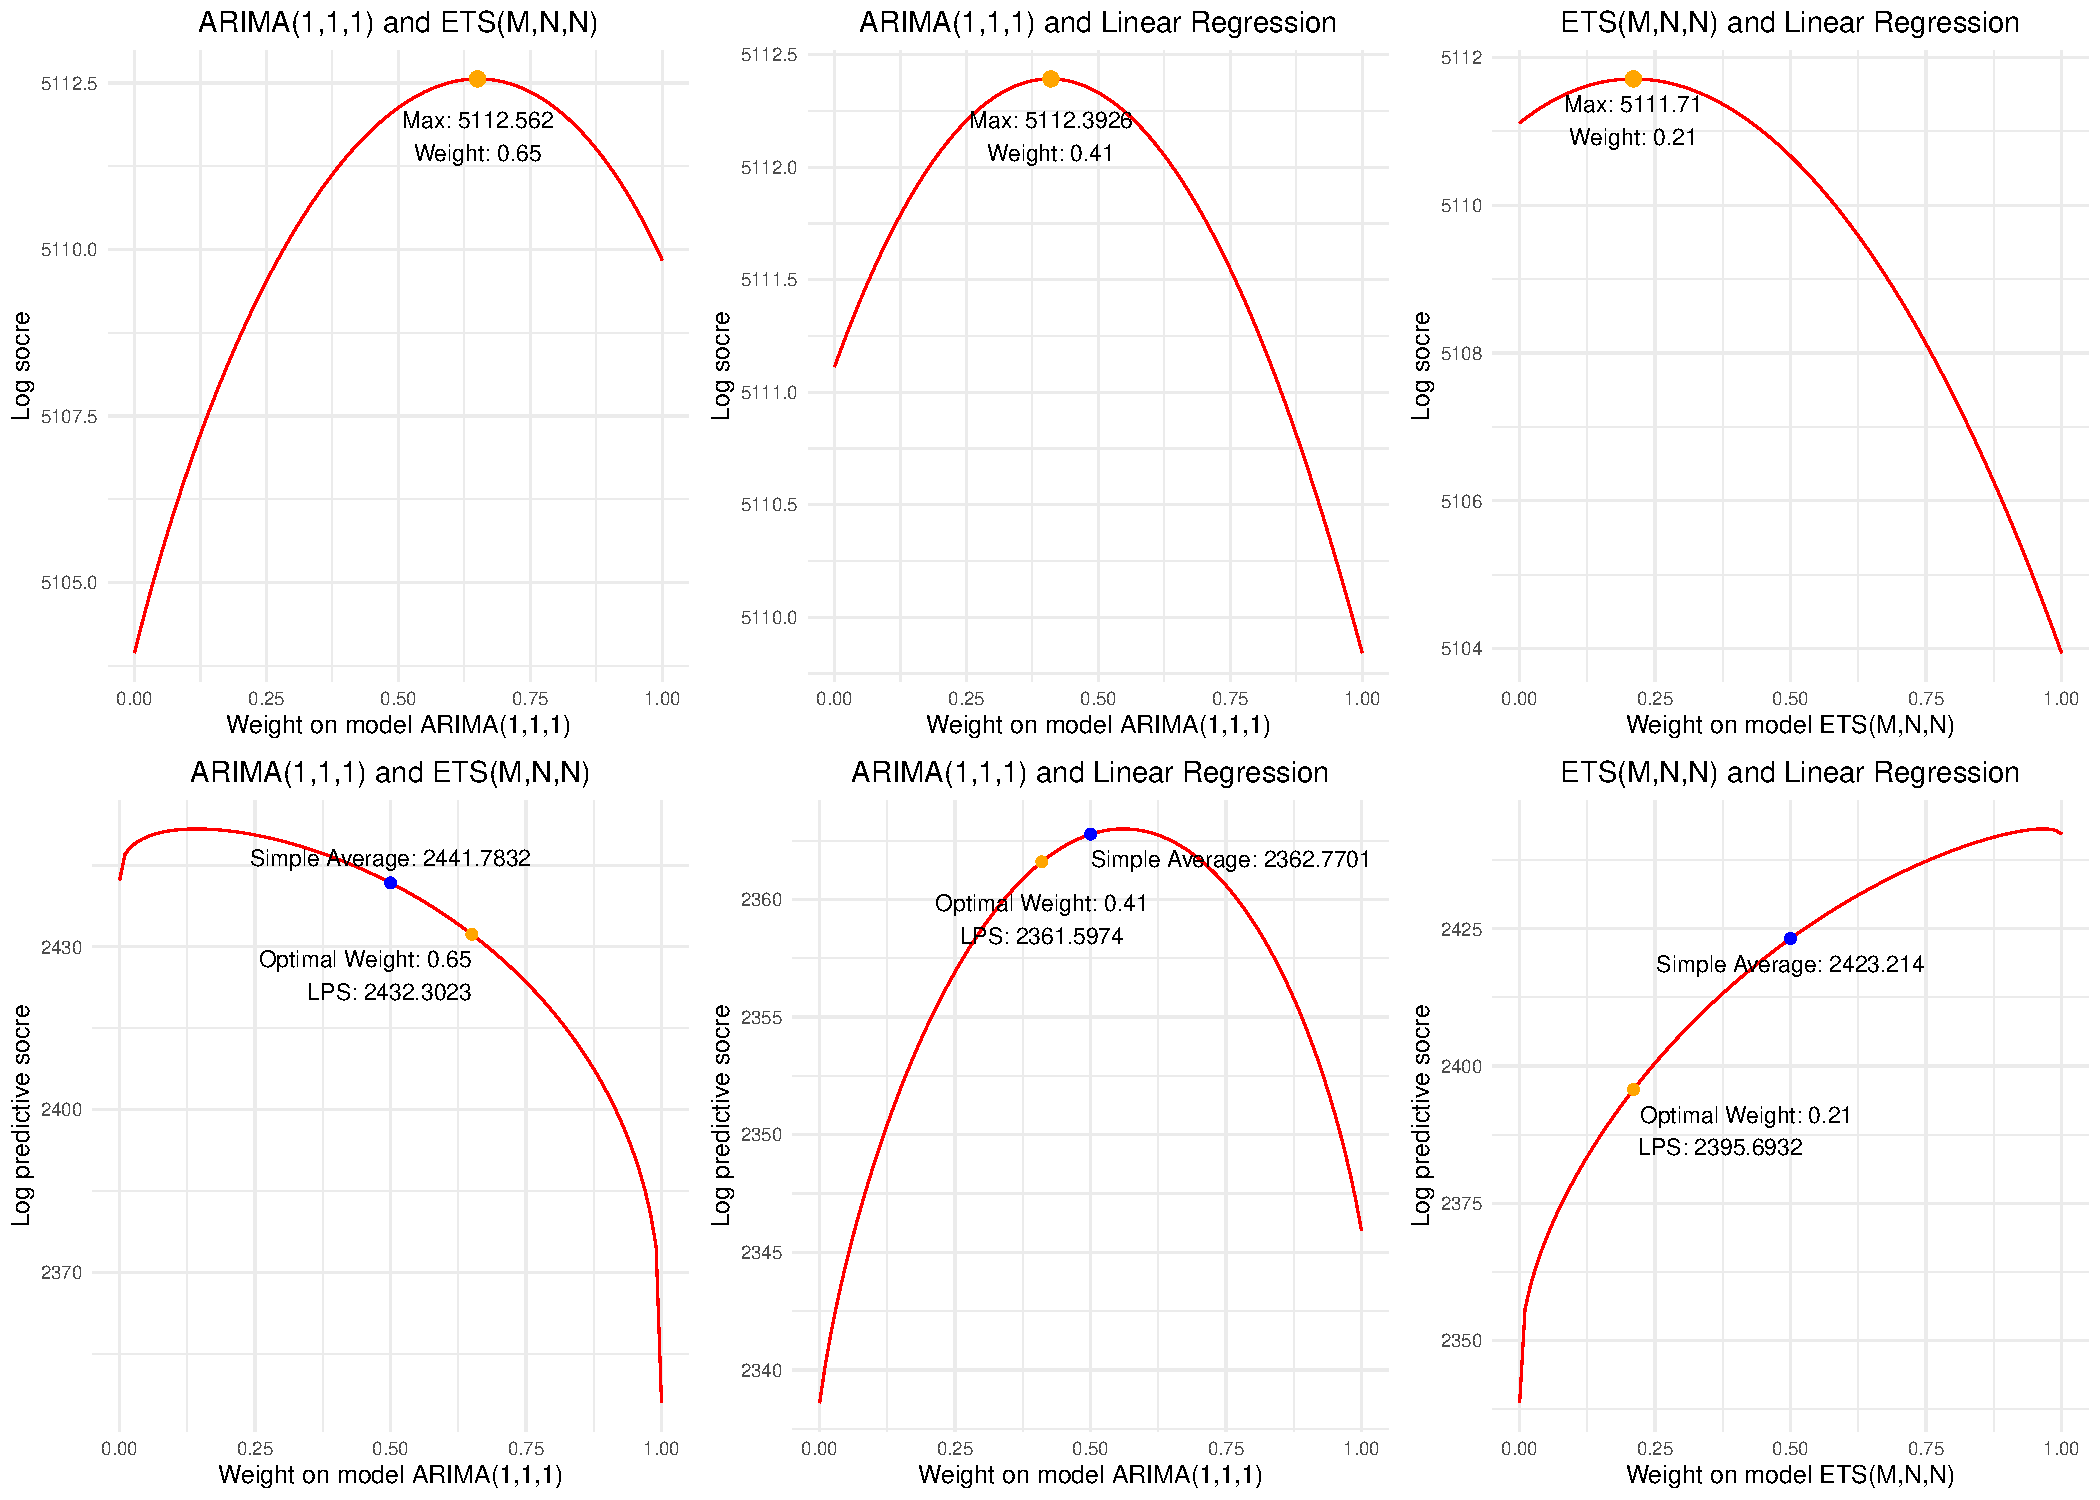
\includegraphics[scale=0.45]{figures/SP500_nonstationary.pdf}
\caption{Log predictive score of S\&P 500 index predictive densities in two-model pools over the in-sample (top) and out-of-sample (bottom) period. Constituent prediction models described in the title. The x-axis represents the weight assigned on the former model of the combination and the y-axis indicates the log predictive score. The orange dot represents the optimal set of weights and the corresponding log predictive score in each case, while the blue dot indicates the forecast performance of the simple averaging method.}
\label{fig:nonstat}
\end{figure}

Figure \ref{fig:nonstat} suggests that the forecast combination puzzle is evidenced in all three cases, where we have the simple average performs better than the optimal combination to different degrees. However, the difference in the log predictive score between two combination methods is varying for each case, and is very likely to be influenced by the in-sample fit performance of constituent models. Relevant values are calculated and presented in Table \ref{tab:comparison1}. It is noticeable that when both models fit the data equally well, i.e., a small difference in the in-sample log score, the prediction accuracy of optimal and simple average approaches is very close to each other. Meanwhile, the optimal forecast combination with a significant gap between the individual in-sample fit ends up performing worse than the mean of forecast densities.

\begin{figure}[ht]
\centering
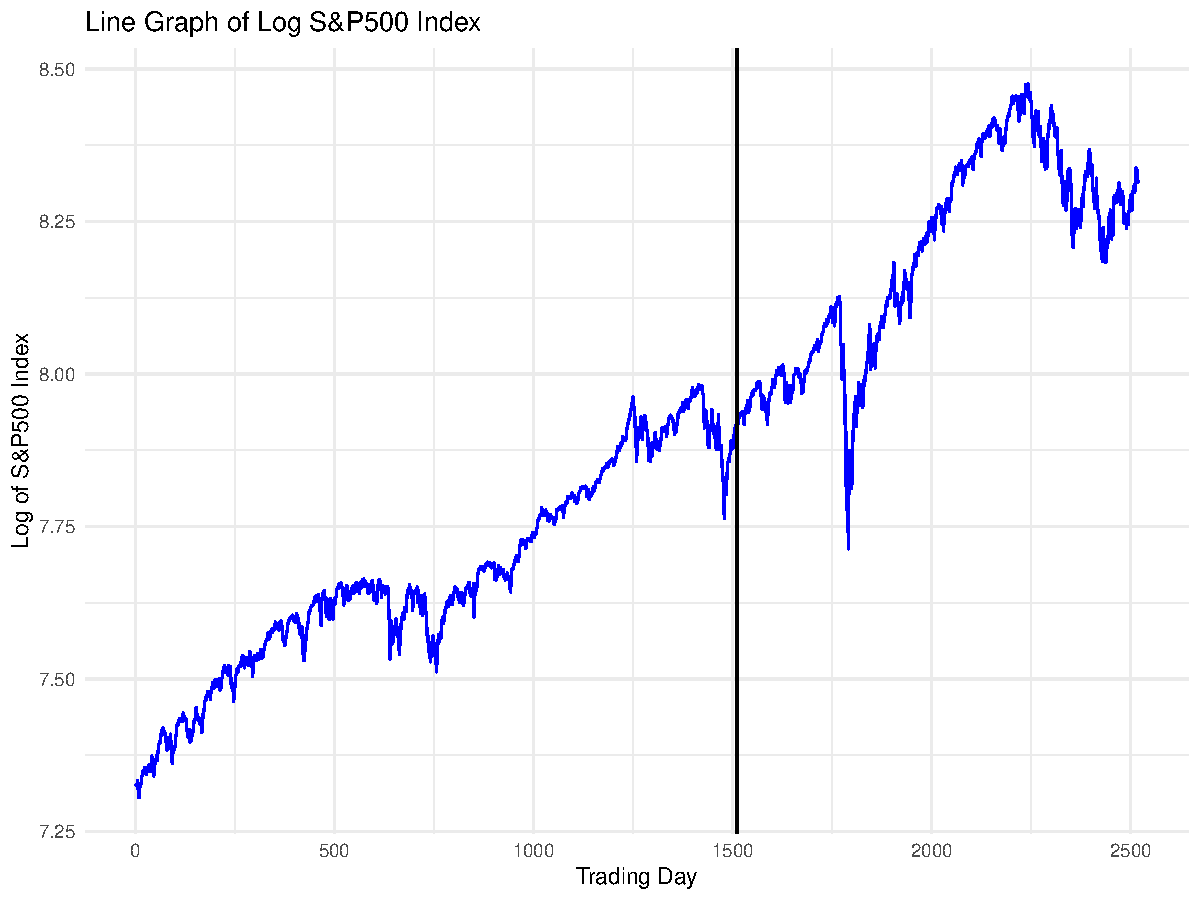
\includegraphics[scale=0.4]{figures/log_linegraph.pdf}
\caption{The black vertical line separates the traning set and the evaluation set. The training set is on the left and the evaluation set is on the right.}
\label{fig:llg}
\end{figure}

One possible explanation could be that the ETS model fits the training set poorly compared to the other two models, while ARIMA and linear regression perform equally well. Based on the specification of ETS(M,N,N), we may argue that it fails to capture the trend component and is therefore a \texttt{Bad} model in the combination. On the other hand, the ARIMA and linear regression can be viewed as \texttt{Good} models.

\hypertarget{stationary-time-series}{%
\subsection{Stationary time series}\label{stationary-time-series}}

Continue with the same dataset, we now take a first difference of the log of S\&P 500 index and then fit this stationary series. A series is said to be stationary when it has constant mean and variance, and its covariance depends on the time interval only. In other words, the entire series should have roughly consistent patterns. Then, it is less likely to get misspecified or poorly fit models.

Consider two candidate models: a Gaussian ARMA(1,1) model and a classical linear regression model with ARMA(1,1) errors. To differentiate with the first linear regression model, it is named as Linear Regression 2 in the combination. Figure \ref{fig:stat} illustrates that two constituent models have a very similar in-sample log score, only 0.0011 difference, and the puzzle is evidenced given only 0.1282 accuracy difference between two forecast combination approaches.

\begin{figure}[ht]
\centering
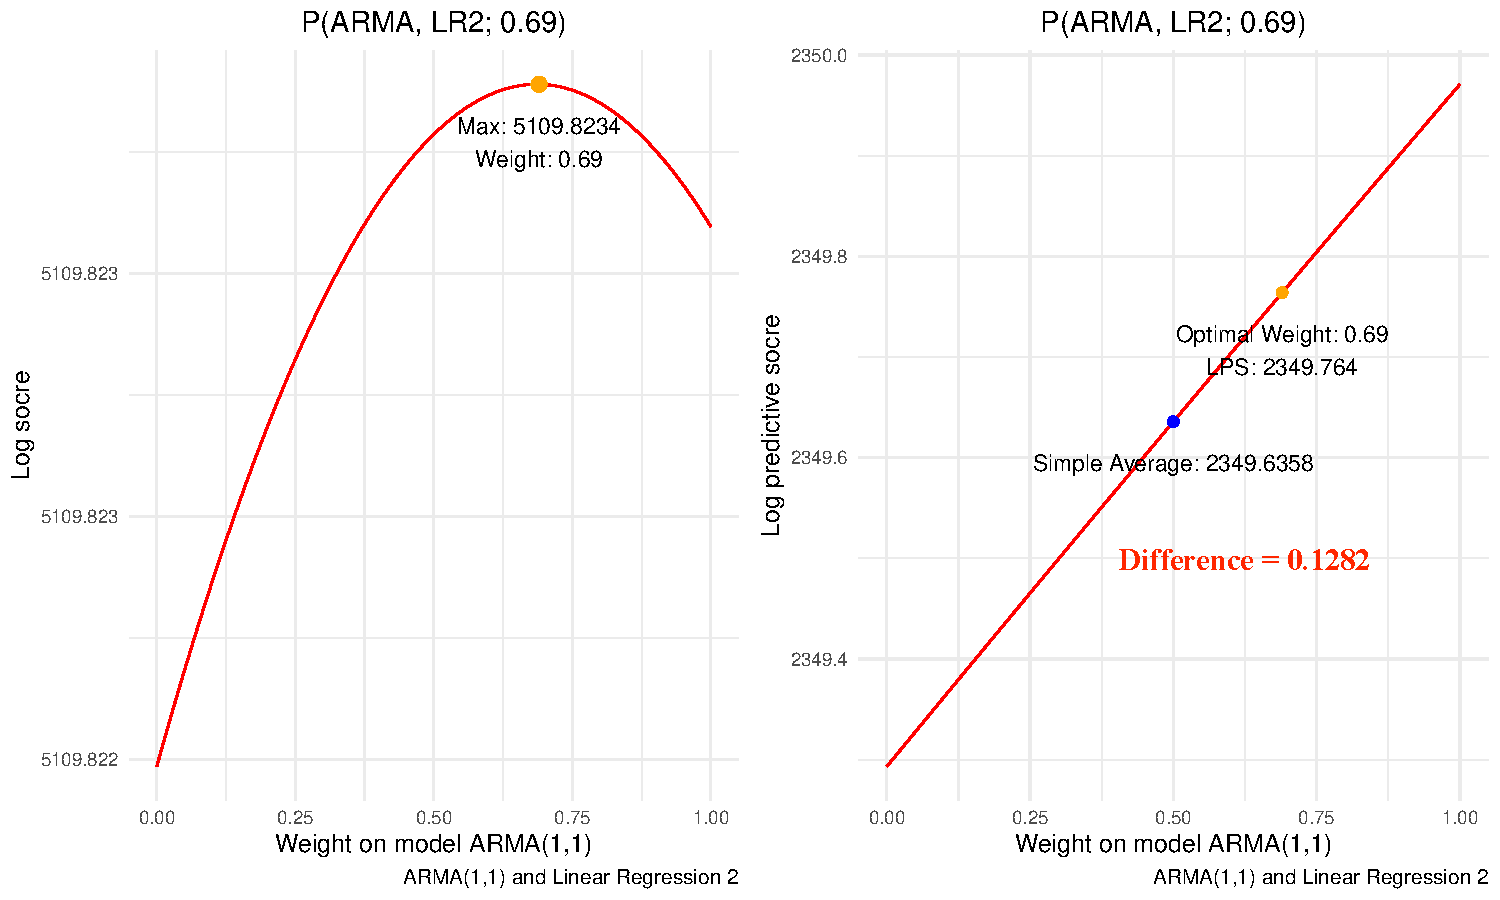
\includegraphics[scale=0.6]{figures/SP500_stationary.pdf}
\caption{Log predictive score of S\&P 500 index predictive densities in two-model pools over the in-sample (left) and the out-of-sample (right) period. The x-axis represents the weight assigned on the ARMA(1,1) model and the y-axis indicates the log predictive score. The meanings of colored dots remain the same as before.}
\label{fig:stat}
\end{figure}

This Section \ref{sp500} provides a little empirical evidence for our initial conjecture. When both models fit the data well, i.e., they are \texttt{Good} models, then the average density forecast performs almost the same as or slightly better than the optimal density forecast combination, indicating the presence of the forecast combination puzzle. If one model is \texttt{Bad} and the other is \texttt{Good}, then, at least, the puzzle can be evidenced.

\hypertarget{pure-time-series-with-seasonality}{%
\section{Pure time series with seasonality}\label{pure-time-series-with-seasonality}}

With the purpose of further examining the speculations, we now use a quarterly dataset to explore the relationship between the forecast combination puzzle and the model fit. More specifically, we would like to investigate cases when models are both correctly specified (good) or both misspecified (bad). To make our life easier, we produce point forecasts and evaluate point combinations with MSFE.

The data considered is the quarterly total number of unemployed individuals (in thousands) from 1985 Q1 to 2023 Q1, retrieved from the Australia Bureau of Statistics \autocite{ABS}. It has a total of 153 (\(T\)) observations and is slit into two sets in proportion. Same as before, the first 60\% of the data (\(R = 91\)), as the in-sample period, is used to estimate all unknown parameters. The rest 40\% (\(P = 62\)) is the out-of-sample period for the forecast performance evaluation. Also, we use the natural logarithm of the total number of unemployment to reduce the level of variability in the series.

\hypertarget{correctly-specified-models}{%
\subsection{Correctly specified models}\label{correctly-specified-models}}

To ensure compatibility with seasonal component, we propose the Seasonal ARIMA (SARIMA) model and the ETS model: ARIMA(2,0,2)(0,1,1){[}4{]} with drift and ETS(A,A,A). The SARIMA is simply an ARIMA model with extra seasonal component. The first parenthesis is same as before. The second parenthesis represents the seasonal AR, integrated, and MA components respectively, separately by the comma. The number in the box bracket indicates the number of observations per year, i.e., the seasonal frequency. An intercept is included in the model. In the ETS model, the seasonal part is reflected by \texttt{S} and the third position in the parenthesis. Due to the log transformation, we have additive error, additive trend, and additive seasonality.

The forecast combination puzzle is evidenced when both models are good in Figure \ref{fig:sd}. The optimal forecast point combination has a MSFE of 0.000177 and the simple averaging forecast has a MSFE of 0.000178. The difference between them is negligible. Looking at the in-sample combination plot, two models fit the training set equally well with a difference of 0.0000005319. These results exemplify that two \texttt{Good} models in a two-model pool will close to having the forecast combination puzzle.

\begin{figure}[ht]
\centering
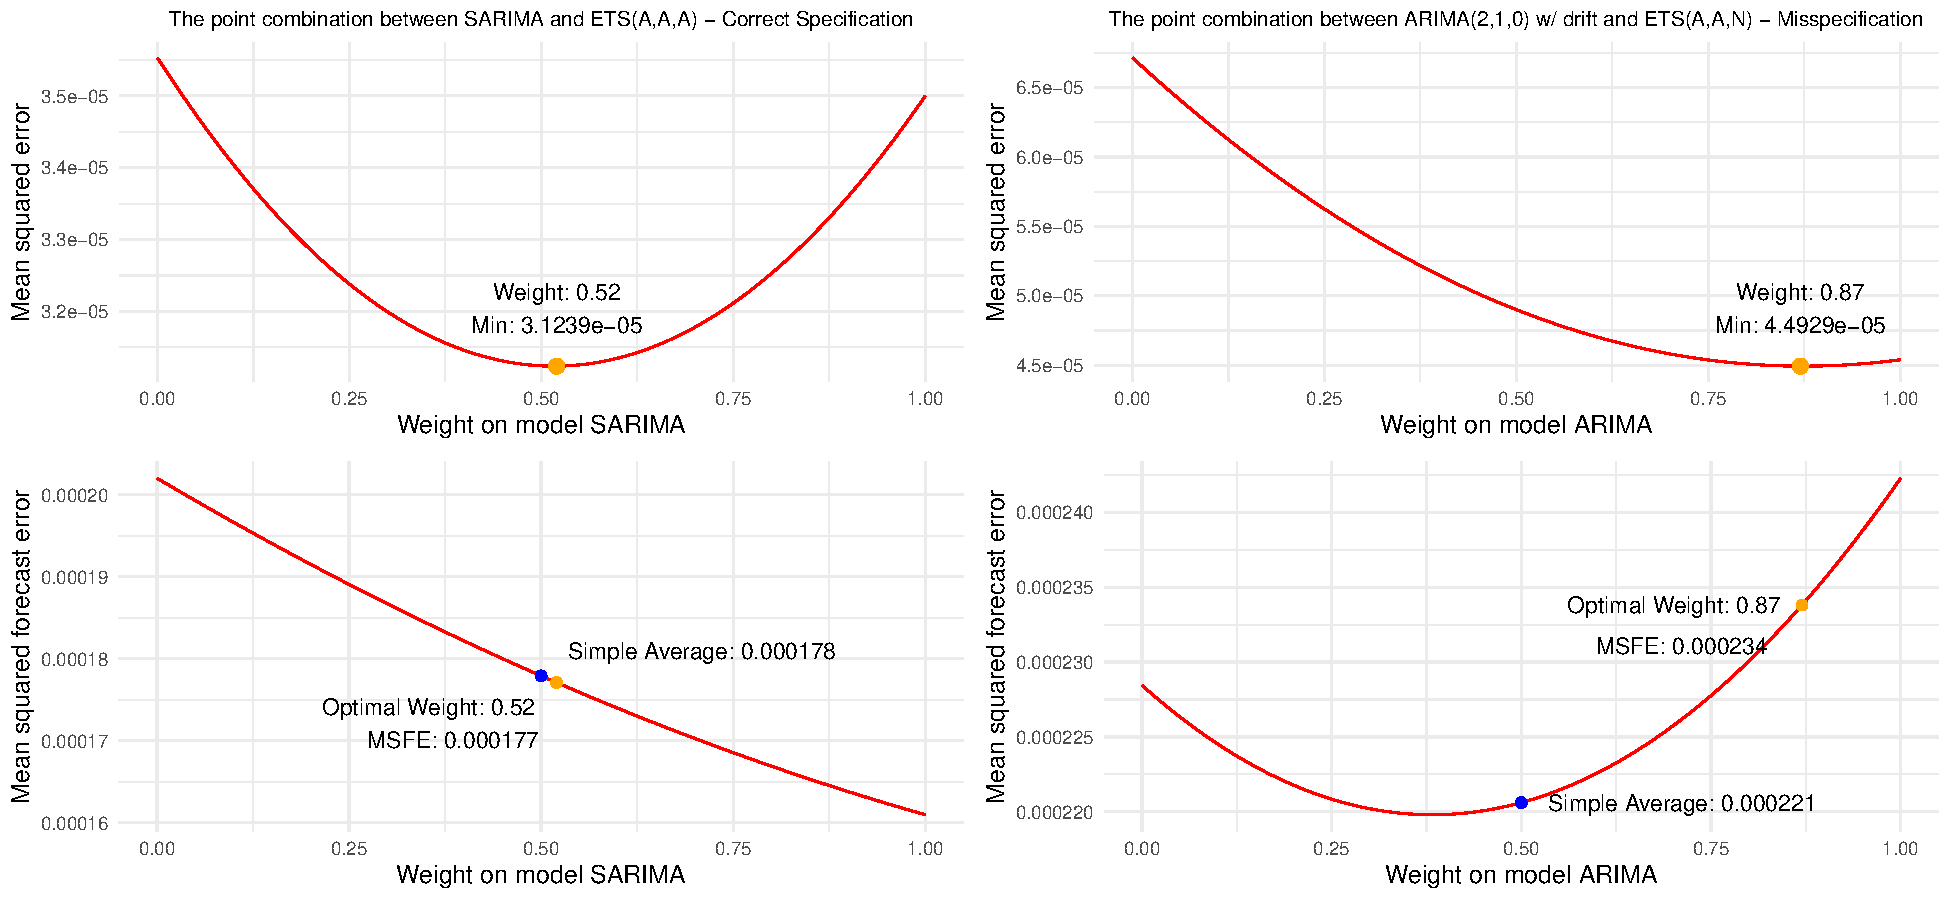
\includegraphics[scale=0.5]{figures/EMPL.pdf}
\caption{MSFE of predictive points in correctly specified (left) and misspecified (right) two-model pools over the in-sample (top) and out-of-sample (bottom) period. The x-axis represents the weight assigned on the first model and the y-axis indicates the value of MSFE. The meanings of colored dots remain the same.}
\label{fig:sd}
\end{figure}

\hypertarget{misspecified-models}{%
\subsection{Misspecified models}\label{misspecified-models}}

One way of proposing a \texttt{Bad} model for a seasonal dataset is deliberately ignoring the seasonality in the model specification. Even so, we still try to fit the training set well with SARIMA and ETS models but only discarding their seasonal components: ARIMA(2,1,0) with an intercept and ETS(A,A,N).

The right column of Figure \ref{fig:sd} illustrates that both models have a similar in-sample performance with a deviation of 0.00002175. Furthermore, Figure \ref{fig:sd} does reveal the forecast combination puzzle, as the simple average performs more superior than the optimal forecast combination with a lower MSFE.

In this case, we may claim that, regardless whether the constituent models capture all the features of the data, as long as they have similar in-sample fit, the forecast combination puzzle will be evidenced. As a result, even we have two \texttt{Bad} models, if they have equivalent in-sample performance, we should expect to have the puzzle.

\hypertarget{simulation-results}{%
\chapter{Simulation Results}\label{simulation-results}}

\hypertarget{pure-cross-sectional-setting}{%
\section{Pure cross-sectional setting}\label{pure-cross-sectional-setting}}

Given that the forecast combination can greatly improve the forecast accuracy, this idea of model combination can also be applied to the cross-sectional setting. A simulated cross-sectional dataset is designed to study how related elements in the linear regression model affect the presence of the puzzle, as well as the performance of density combinations. Compared with empirical data, implementing simulation is easy for us to control things and make any changes we like. At the same time, it is an easy way of validating the conjectures by exploring the puzzle from different aspects. In line with previous notations but in the cross-sectional setting, the subscript \texttt{t} will change to \texttt{i} to represent each individual observation.

\hypertarget{experimental-design}{%
\subsection{Experimental design}\label{experimental-design}}

The true data-generating process (DGP) is assumed to be a classic linear regression model with only two exogenous and correlated regressors, which satisfies all classical assumptions:

\begin{equation}
\label{eqn:DGP}
y_i = \beta_0 + \beta_1 x_{1i} + \beta_2 x_{2i} + e_i, \ \ e_i \stackrel{i.i.d}{\sim} N(\mu_e,\sigma^2_e) \\
\end{equation}

where \(i\) represents each observation.

The initial set-up has 15000 (N) artificial cross-sectional observations generated from \ref{eqn:DGP} with \(E[x_{1i}] = E[x_{2i}] = 0\), \(Var(x_{1i}) = Var(x_{2i}) = 1\), \(Cov(x_{1i}, x_{2i}) = 0.7\), \(\pmb{\beta} = (\beta_0, \beta_1, \beta_2)' = (1,2,2)'\), \(\mu_e = 5\) and \(\sigma^2_e=10\).

Following the methodology in Section \ref{method}, the data will be divided into an in-sample period (roughly 60\%) for estimation and an out-of-sample period for accuracy evaluation. We propose two misspecified models to generate density forecasts with each only contains one of the regressors. Assume Model 1 includes only \(x_{1i}\) as the regressor and the other model, Model 2, includes only \(x_{2i}\) as the regressor. The density forecast combinations will follow the construction of \texttt{two-model} pools and be evaluated by the log score functions.

\begin{figure}[ht]
\centering
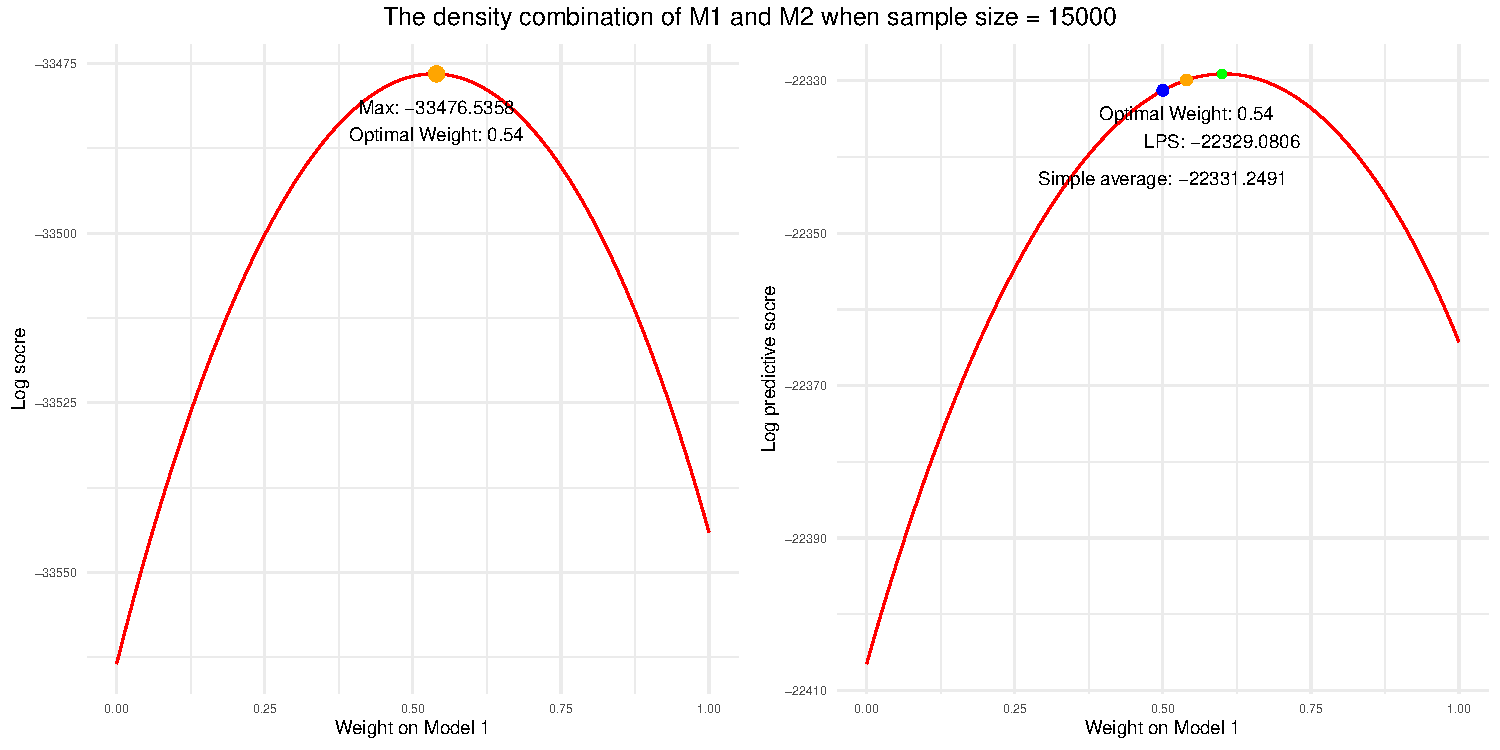
\includegraphics[scale=0.6]{figures/Sample_Size_15000.pdf}
\caption{Two curves refer to the in-sample (left) and out-of-sample (right) performance of density combinations with artificial cross-sectional data under the initial set-up. The x-axis represents the weight assigned on Model 1 and the y-axis indicates the log score for each density combination. The orange dot represents the optimal set of weights and the corresponding log predictive score in each case, while the blue dot indicates the forecast performance of the simple averaging method. The green dot, as a reference, refers to the maximum point of the out-of-sample curve.}
\label{fig:ss15000}
\end{figure}

Figure \ref{fig:ss15000} clearly reflects that when the sample size is large enough, the simple average of predicted densities, indicated by the blue dot, can retain the forecast accuracy with a small difference in the log predictive score, compared with the optimal combination indicated by the orange dot. This is an evidence of facing forecast combination puzzle. Given the puzzle, we can change the true value of relevant elements one at a time while holding all others constant, and then summarize the conditions under which the puzzle is likely to be evidenced.

\begin{itemize}
\tightlist
\item
  \bf{Sample Size}
\end{itemize}

\begin{figure}[ht]
\centering
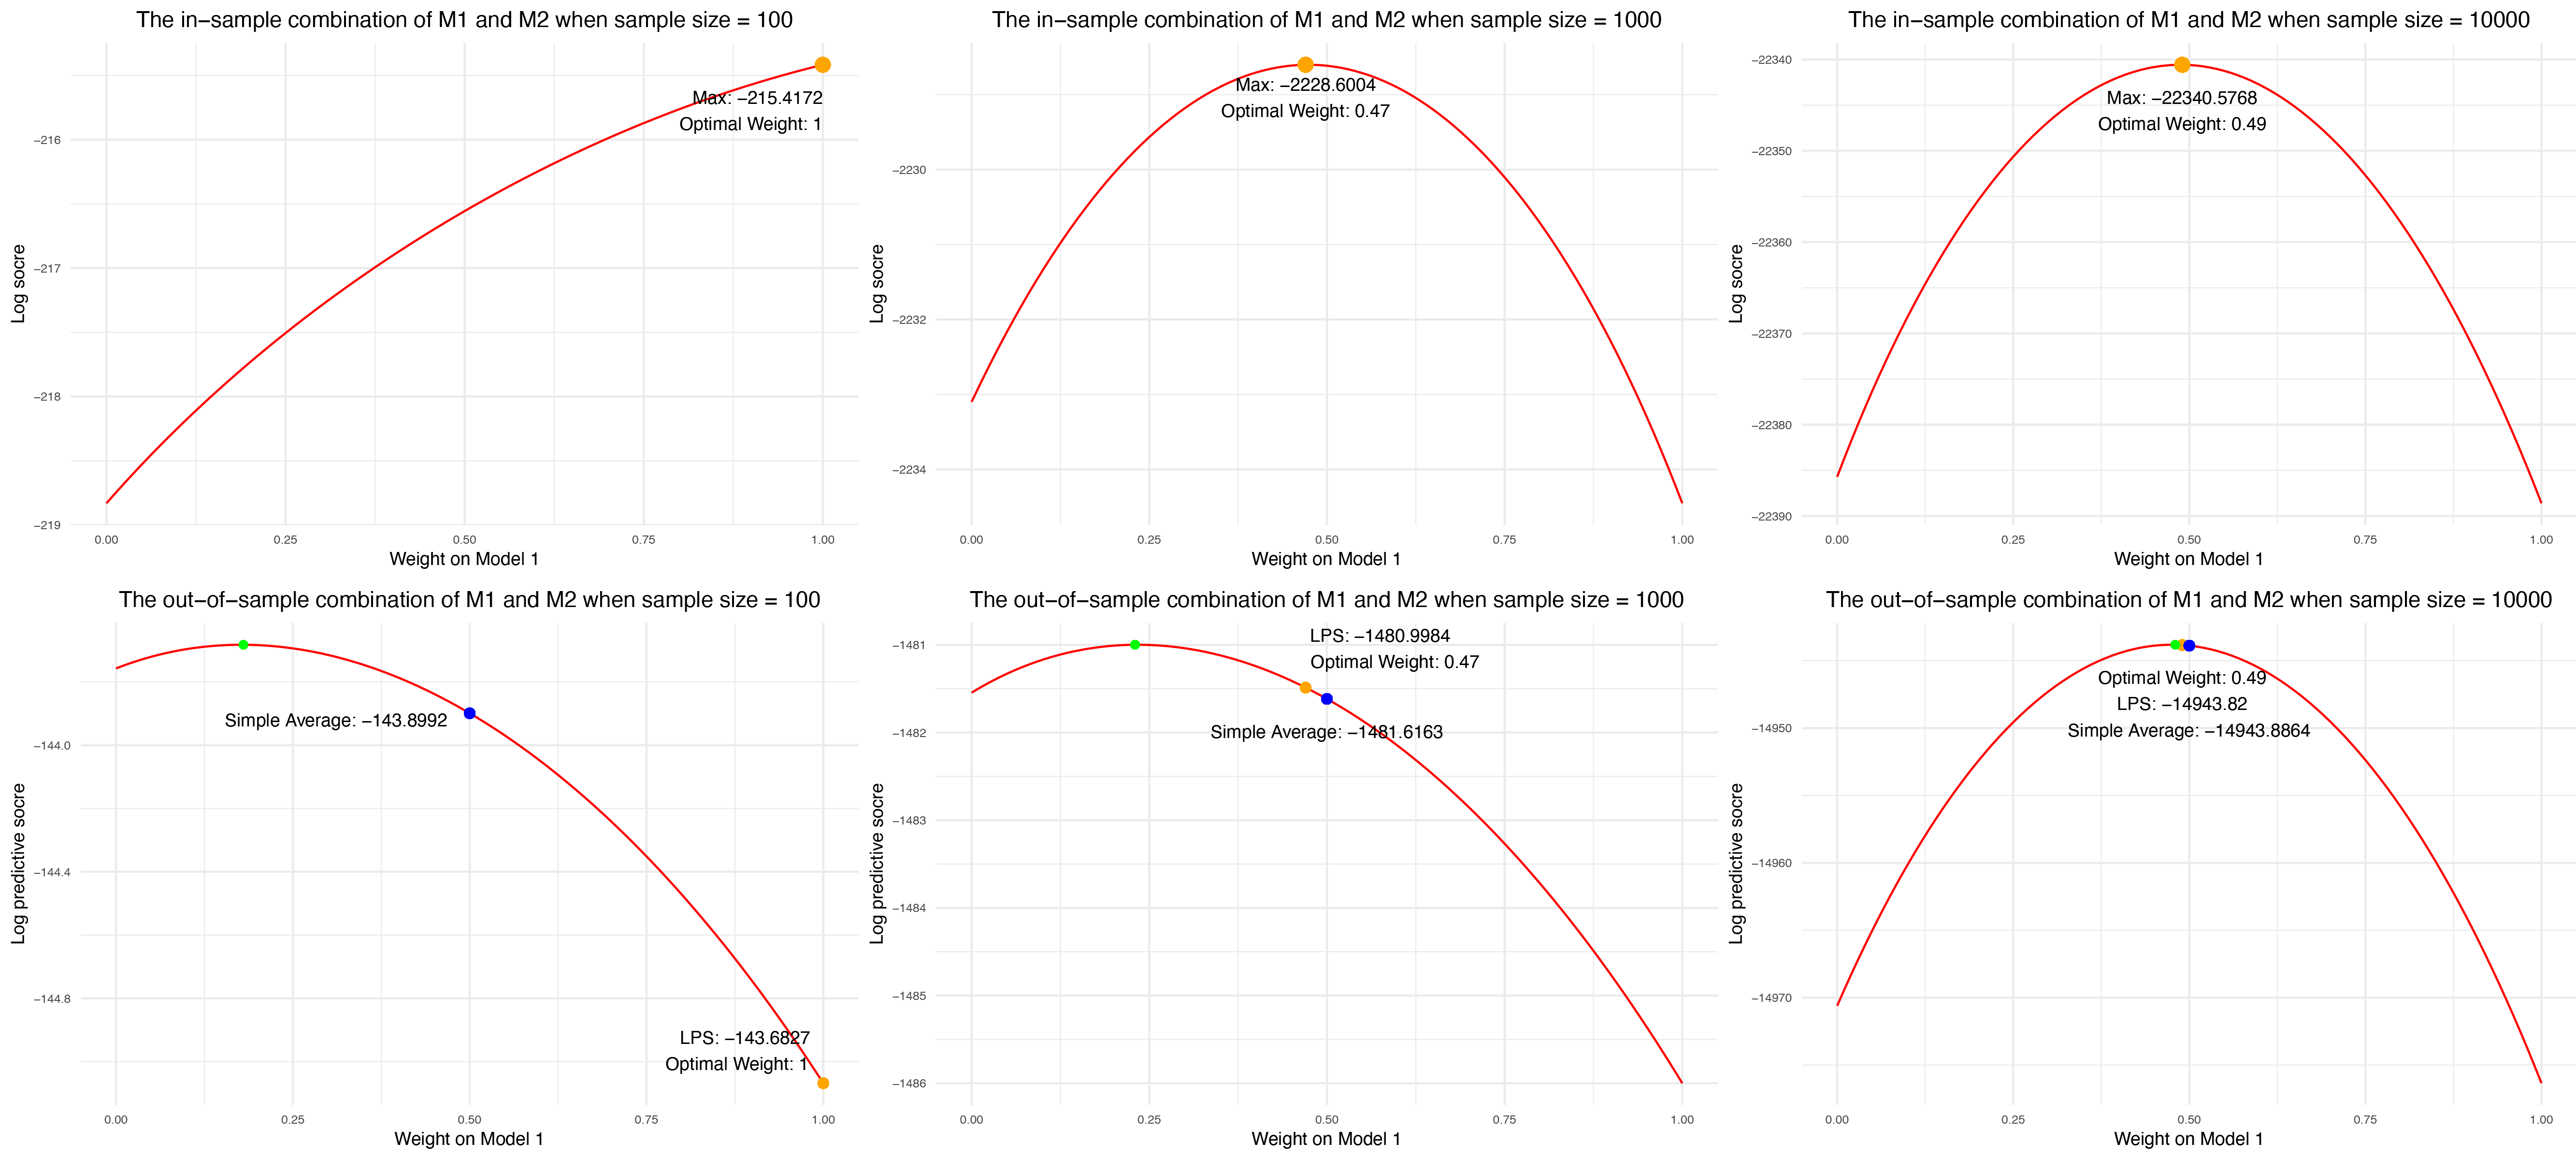
\includegraphics[scale=0.35]{figures/Sample_Size_100-10000.png}
\caption{Three columns refer to cases when $N=100$, $N=1000$, and $N=10000$ respectively while keeping all others constant as the initial set-up. The top graphs represent the in-sample combination performance and the bottom graphs represent the out-of-sample combination accuracy. The meanings of colored dots are the same as those in Figure \ref{fig:ss15000}.}
\label{fig:ss}
\end{figure}

First, it is notable that, in Figure \ref{fig:ss}, the performances of in-sample and out-of-sample combinations have completely different shapes or features when \(N=100\) but are gradually similar when \(N=1000\) and \(N=10000\). In the \(N=100\) case, we completely prefer Model 1 to fit the training set, however, the Model 1 becomes the worse choice for the test set. Thus, the averaged density forecast performs much better than the combination recommended by the optimal weight. This implies that the model combination which fits the in-sample well does not necessarily generate better forecasts when the sample size is small. Second, the forecast accuracy of optimal combination and that of simple averaging are getting closer when the sample size increases, which indicates the presence of the forecast combination puzzle. Roughly, the puzzle becomes noticeable when the sample size is larger than 500.

When we have a small dataset, it is not representative of the whole population, so the model estimation involves more randomness and is highly influenced by potential outliers. There is also a possibility of overfitting the training set when the training and test sets have distinct patterns. Therefore, given a large enough dataset and two equally good models, we are very likely to have the puzzle.

\begin{itemize}
\tightlist
\item
  \bf{Magnitude and Sign of $\pmb{\beta}$}
\end{itemize}

Next, the sample size is set to be 10000 so that it is large enough to reveal the puzzle. Consider the change in magnitude and sign of \(\beta_1\) and \(\beta_2\).

\begin{figure}[ht]
\centering
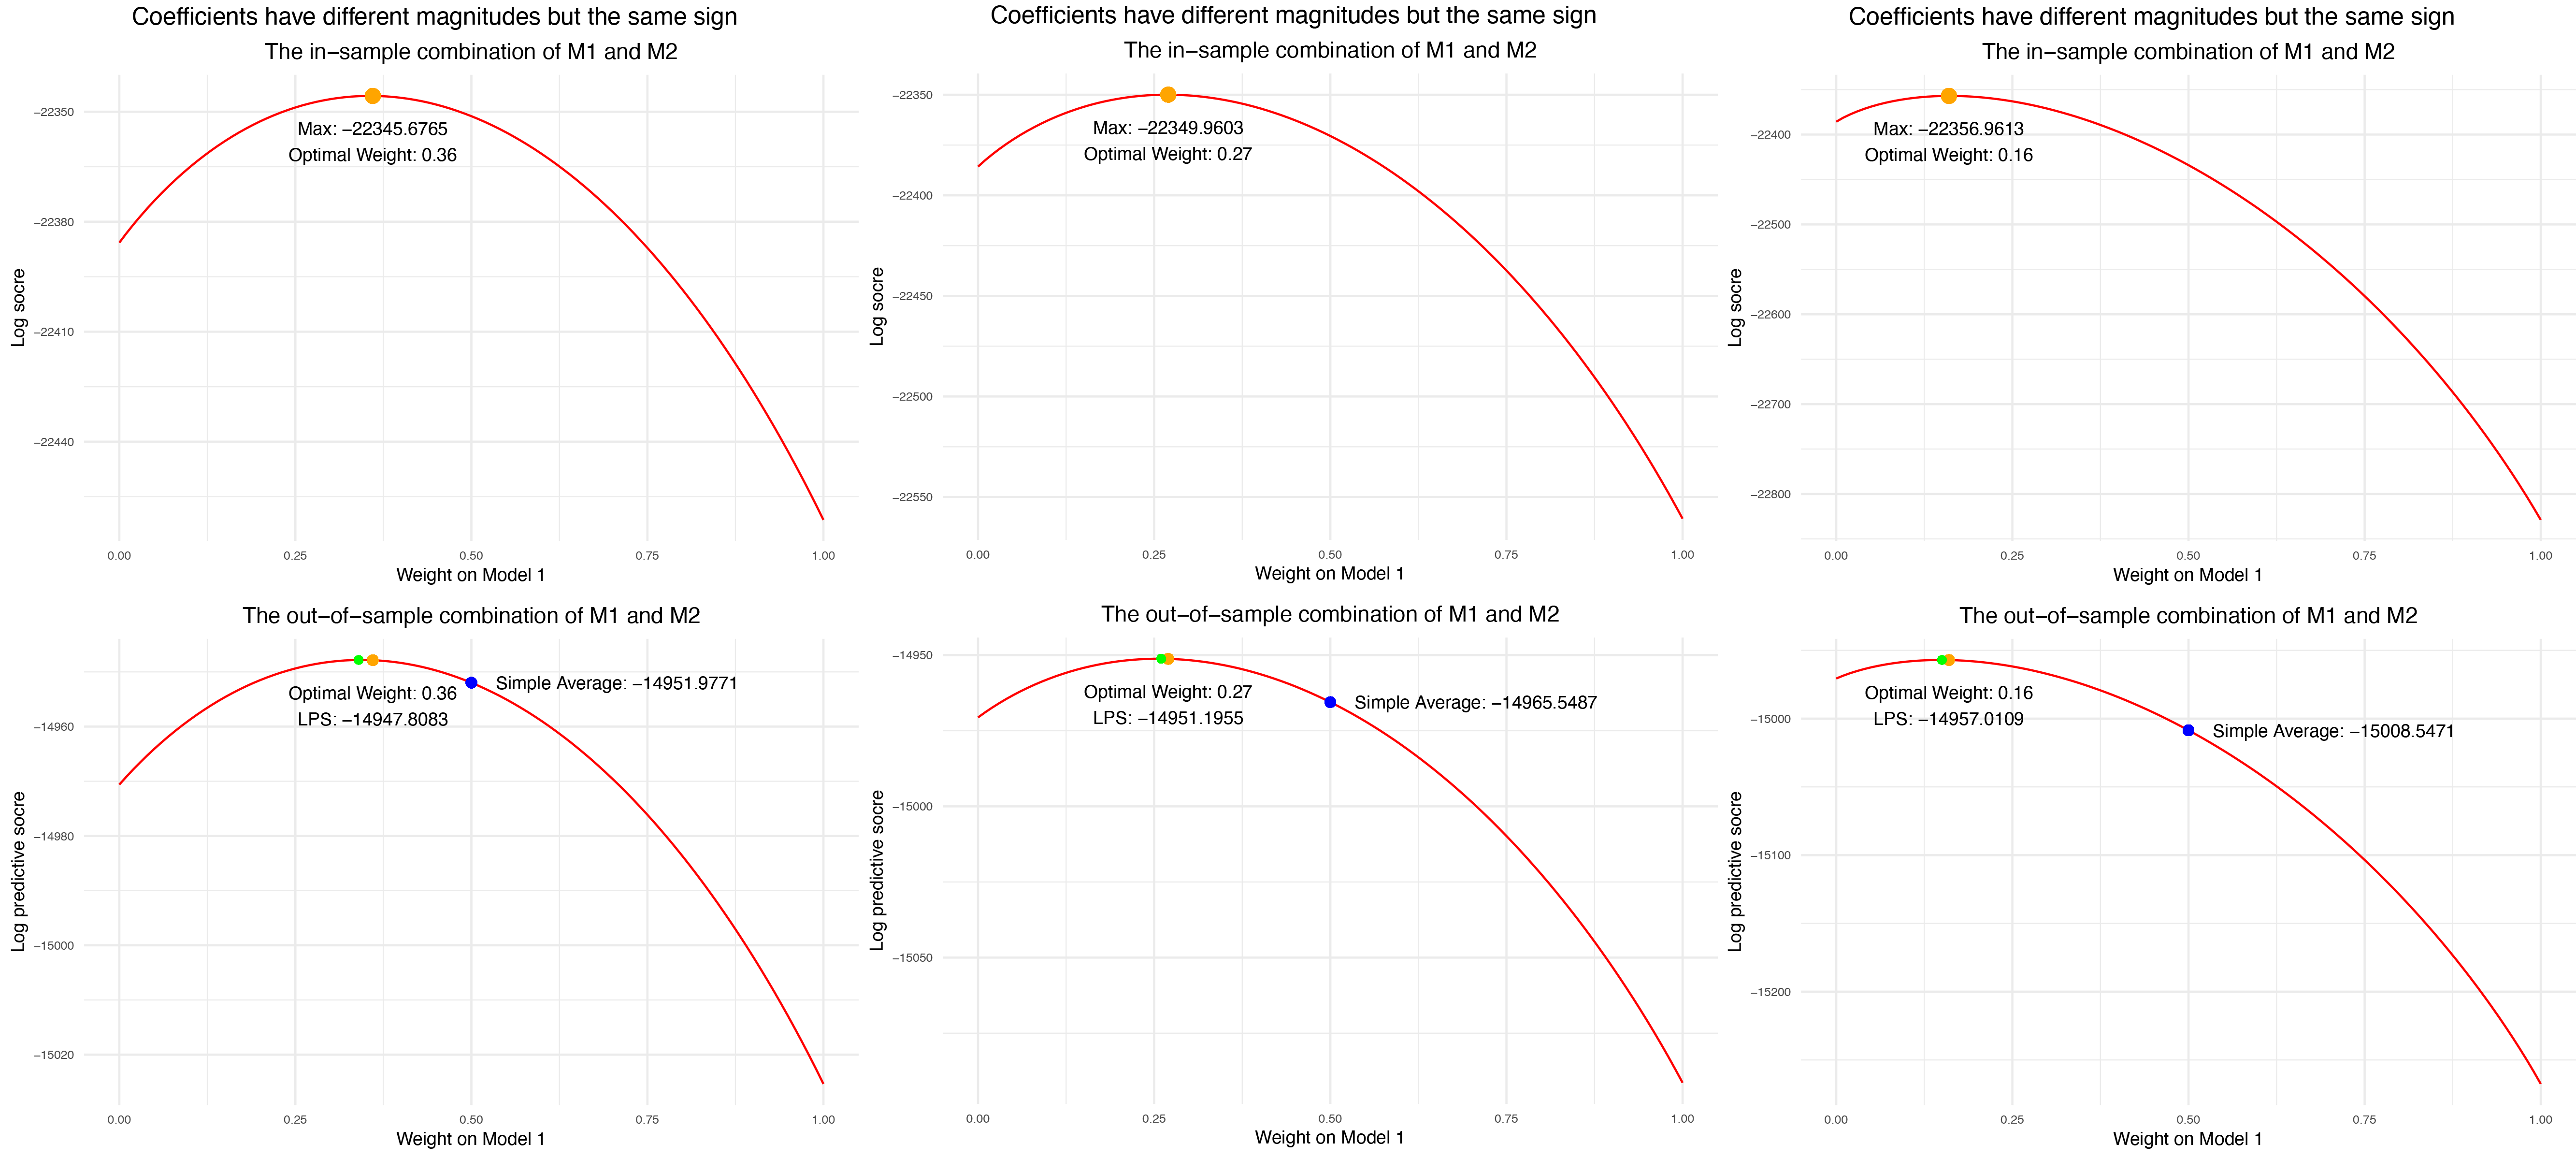
\includegraphics[scale=0.35]{figures/Beta_diff_mag.png}
\caption{In this case, $\beta_1$ and $\beta_2$ have the same sign but different magnitudes. The first column refers to $\beta_1=2$ and $\beta_2=3$, the second column refers to $\beta_1=2$ and $\beta_2=4$, and the third column refers to $\beta_1=2$ and $\beta_2=6$.}
\label{fig:magnitude}
\end{figure}

Based on the results shown in Figure \ref{fig:magnitude}, the puzzle is highly sensitive to the absolute difference between two parameters. If the absolute difference is large enough, generally more than half of the smaller coefficient, it is hard to observe the puzzle and the optimal combination always wins with a higher log predictive score. The larger the absolute difference, the bigger the difference of two log predictive scores.

In the linear regression analysis, the magnitude of each coefficient represents the influence size of each regressor on the dependent variable. A large coefficient means that a change in the corresponding regressor affects the dependent variable more in magnitude. Knowing this, it is reasonable to observe that the Model 1 has a decreasing weight in the optimal combination from left to right in Figure \ref{fig:magnitude}. The effect of \(x_{2i}\) on \(y_i\), \(\beta_2\), is relatively larger than the effect of \(x_{1i}\) on \(y_i\), \(\beta_1\), so the Model 2 with \(x_{2i}\) only should be weighted higher in the combination.

\begin{figure}[ht]
\centering
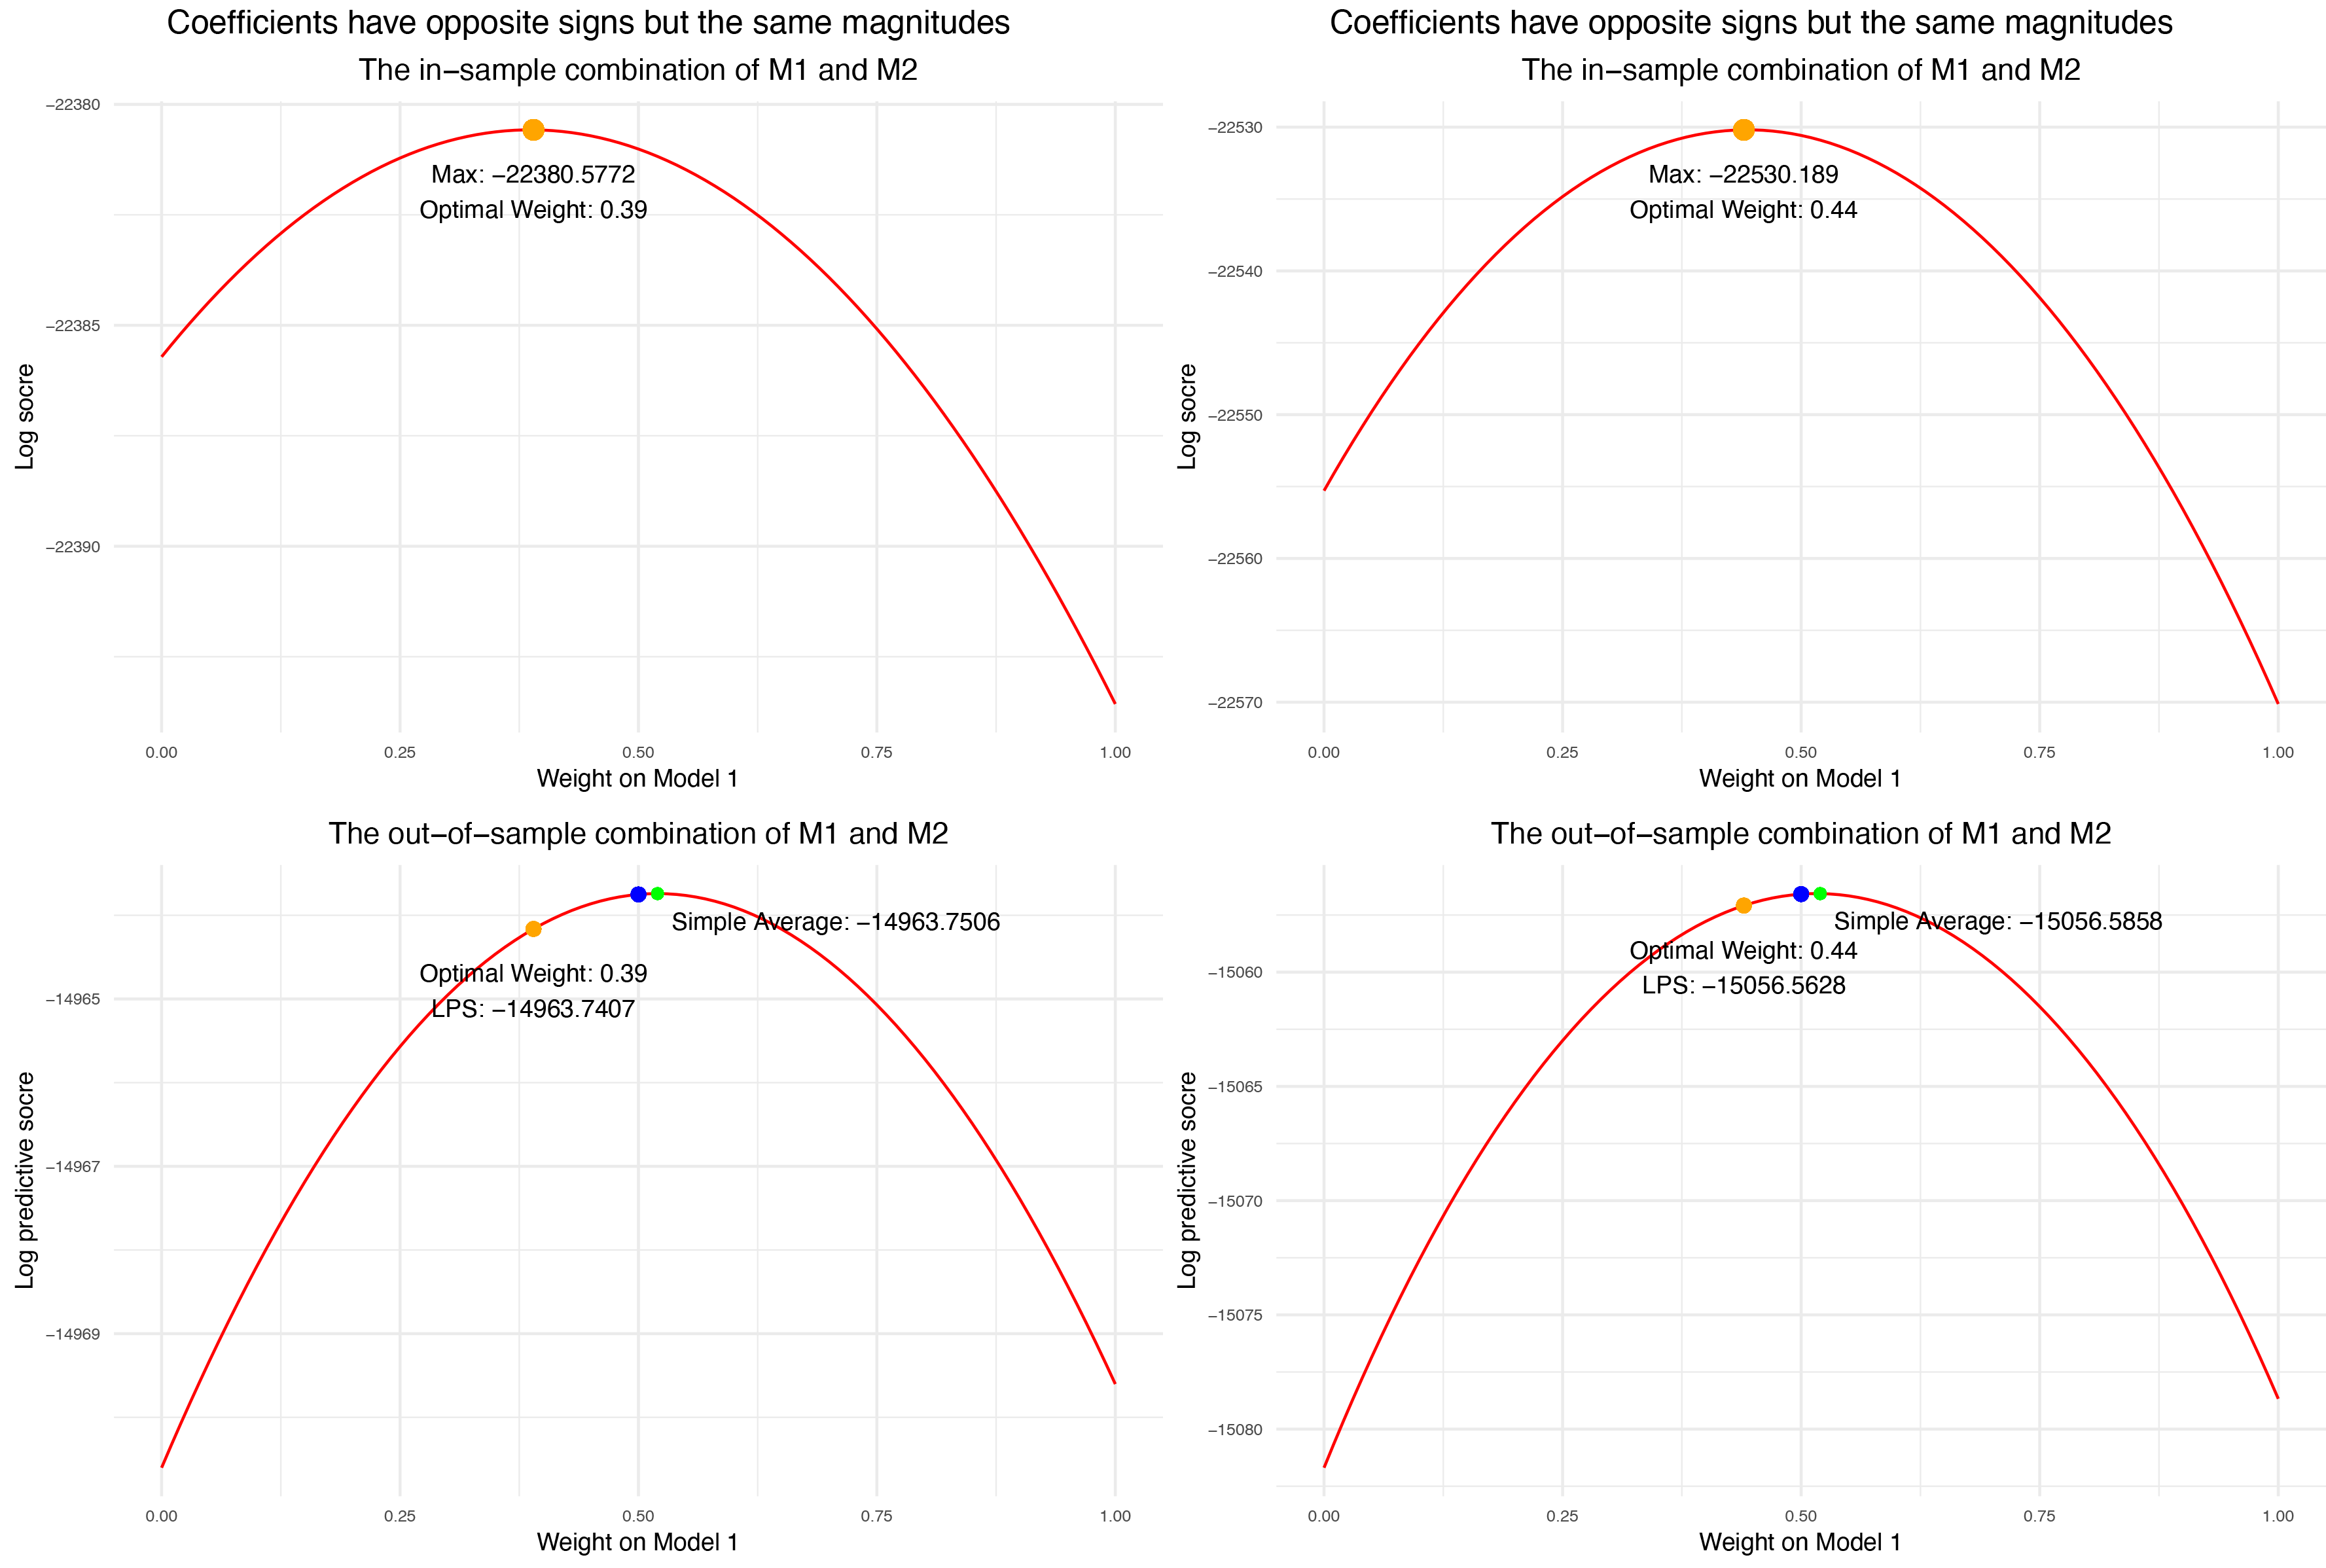
\includegraphics[scale=0.55]{figures/Beta_diff_sign.png}
\caption{$\beta_1$ and $\beta_2$ have the same magnitude but different signs, i.e. $\beta_1=-\beta_2$. The first column considers the case when $\beta_1=2$ and $\beta_2=-2$ and the second column considers the case when $\beta_1=4$ and $\beta_2=-4$.}
\label{fig:sign}
\end{figure}

Figure \ref{fig:magnitude} illustrate that when \(\beta_1\) and \(\beta_2\) only have opposite signs, the puzzle seems to be insensitive. In both cases, the optimal combination and simple averaging forecast have very similar log predictive scores, which is a strong evidence of the puzzle. Meanwhile, two regressors have the same effect in magnitude on \(y_i\), therefore, the weight should be equally assigned in rough. We also notice that the accuracy of the optimal prediction combination can be improved by having higher absolute values of the coefficients. This makes regressors to have larger and more certain impacts on \(y_i\), which is substantiated by the above case.

\begin{itemize}
\tightlist
\item
  \bf{Variance of regressors}
\end{itemize}

\begin{figure}[ht]
\centering
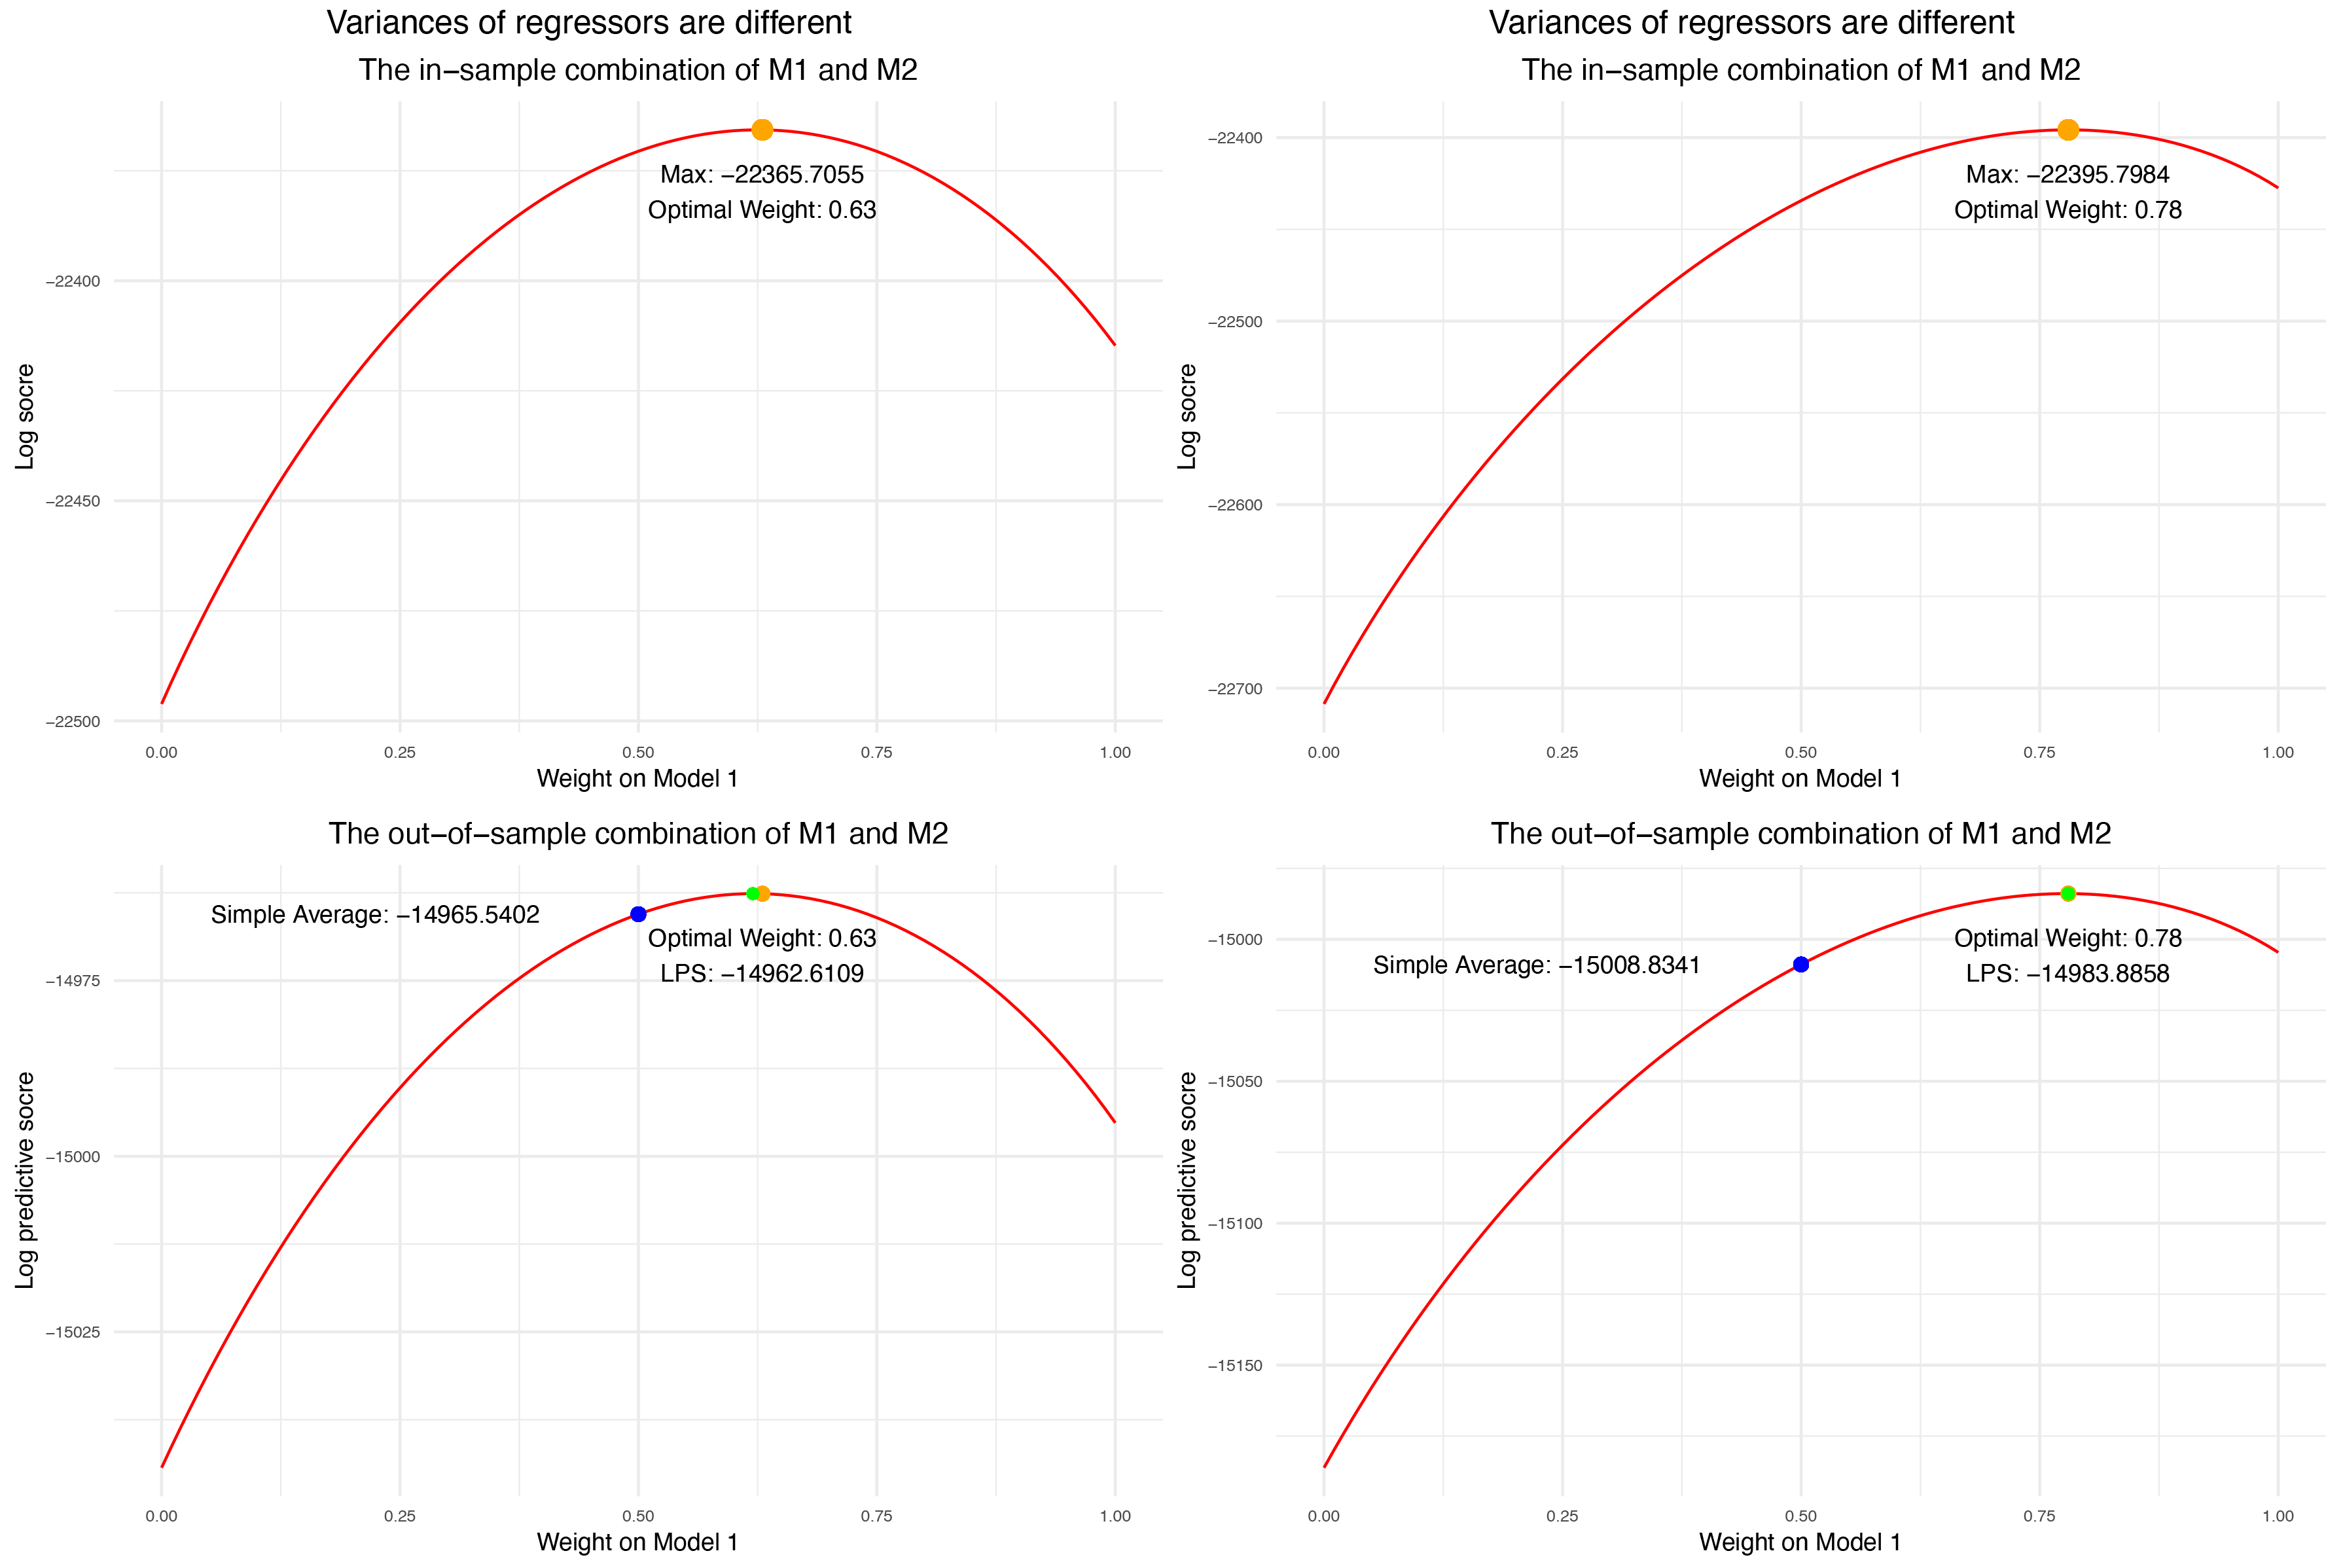
\includegraphics[scale=0.55]{figures/x_var.png}
\caption{The first column refers to the case when $Var(x_{1i}) = 2$ and $Var(x_{2i}) = 1$. The second column refers to the case when $Var(x_{1i}) = 4$ and $Var(x_{2i}) = 1$.}
\label{fig:xvar}
\end{figure}

First thing to note from Figure \ref{fig:xvar} is that there is no forecast combination puzzle when the variances of two regressors are different. When the difference becomes larger, the gap of the forecast accuracy between the optimally combined forecast and the simple average increases as a consequence. Since \(x_{1i}\) has a larger variance than \(x_{2i}\), the variation of \(y_i\) can be explained more by the Model 1, which includes \(x_{1i}\), than the Model 2, which only consists of \(x_{2i}\). This also makes the Model 1 to have more weight in the optimal combination. Besides, the in-sample accuracy between two models is significant, leading the puzzle not to be evidenced, based on the results in Section \ref{sp500}.

\hypertarget{discussion}{%
\chapter{Discussion}\label{discussion}}

\hypertarget{section}{%
\section{}\label{section}}

\hypertarget{timeline-of-future-research}{%
\section{Timeline of Future Research}\label{timeline-of-future-research}}

\begin{table}[ht]
  \centering
  \caption{Updated Research Plan}
  \scalebox{0.8}{
    \begin{tabular}{lll}
    Time        &     Objectives    &     Progress \\
    \midrule
    May - June  & Investigated the puzzle in cross-sectional data and literature review    & Finished \\
    July        & Examined the effect of model specifications on the puzzle with a quarterly data   & Finished \\
    August      & Learning the forecast accuracy tests and drafting thesis    & In progress \\ 
    September   & Applying forecast accuracy tests with time series and considering limitations   & Not started \\
    October     & Working on thesis and final presentation    & Not started \\
    \end{tabular}
  }
\end{table}

\hypertarget{conclusion}{%
\chapter{Conclusion}\label{conclusion}}

Working in the two-model pools provides an opportunity of exploring a variety of situations in a short period of time. The next challenging step should naturally be to investigate the multiple forecasts combination, and we leave it to future research.

\appendix

\hypertarget{appendix}{%
\chapter{Appendix}\label{appendix}}

Exact formulas and explanations of these models can be found in \textcite{fpp3}. The formula of the conditional variance for the ETS models in this case is discussed in Chapter 6.3 of \textcite{HKOS08}. All codes are performed in R Statistical Software (version 4.2.1 (2022-06-23)). The packages used are \texttt{tidyverse} \autocite{tidy19}, \texttt{dplyr} \autocite{dplyr23}, and \texttt{fpp3} \autocite{fpp23}.

\hypertarget{model-specification}{%
\section{Model Specification}\label{model-specification}}

\hypertarget{nonstationary-sp-500-index}{%
\subsection{Nonstationary S\&P 500 Index}\label{nonstationary-sp-500-index}}

\begin{enumerate}
\def\labelenumi{\arabic{enumi}.}
\item
  ARIMA(1,1,1) model with an intercept of the natural logarithm of S\&P 500 index.
  \begin{equation*}
  log(y_t) = c + log(y_{t-1}) + \phi_1\big[log(y_{t-1})-log(y_{t-2})\big] + \epsilon_t + \theta_1\epsilon_{t-1}
  \end{equation*}
\item
  ETS(M,N,N) model of the natural logarithm of S\&P 500 index.
  \begin{align*}
  log(y_t) &= \ell_{t-1} (1+\epsilon_t) \\
  \ell_t &= \ell_{t-1} (1+\alpha \epsilon_t) \\
  \end{align*}
\item
  A classical linear regression model of the natural logarithm of the S\&P 500 index and ARIMA(1,0,0) errors.
  \begin{align*}
  log(y_t) &= \beta_0 + \beta_1 t + u_t \\
  u_t &= \phi_1 u_{t-1} + \epsilon_t
  \end{align*}
\end{enumerate}

The error term, \(\epsilon_t\), in each model is assumed to be independent and normally distributed with a zero mean and a constant variance.

\printbibliography[title={Reference}]




\end{document}
